\documentclass[11pt]{beamer}

\usepackage[utf8]{inputenc}
\usepackage[english]{babel}
\usepackage{amsmath}
\usepackage{amsfonts}
\usepackage{amssymb}
\usepackage{tikz}
\author[shortname]{Domagoj Fizulic \and Felix Gutmann}

\title{Unsupervised Learning in Decision Making}
%\setbeamercovered{transparent} 
%\setbeamertemplate{navigation symbols}{} 
%\logo{} 
%\institute{} 
%\date{} 
\subject{Master Project} 
\begin{document}
	
\frame{\titlepage}

\begin{frame}{Introduction}
\setbeamertemplate{itemize items}[circle]
\begin{itemize}
	\item Introduction
	\item Reinforcement learning and simulation
	\item Experiment Data 
	\item Experiment results
\end{itemize}
\end{frame}
	
\begin{frame}{Reinforcement Learning}
	\framesubtitle{Multi arm bandit experiment}
	\setbeamertemplate{itemize items}[circle]
	\begin{figure}
		\includegraphics[scale=0.3]{Pictures/p2.png}
	\end{figure}

	\begin{itemize}
		\item Choose sequentially from set of choices 
		\item Objective: Maximize revenues
	\end{itemize}
\end{frame}

\begin{frame}{Reinforcement Learning}
\setbeamertemplate{itemize items}[circle]
\framesubtitle{Essential functions and agent modeling}
Softmax Decision Function:
\begin{align*}
P(a)_{t+1} &= \frac{e^{\frac{Q_t(a)}{\tau}}}{\sum_{i}^{N} e^{\frac{Q_t(i)}{\tau}}}
\intertext{Update rule for value function of an action:}
Q(a)_{t+1} &= Q(a)_t + \alpha \left[ R(a)_t -  Q(a)_t	 \right]
\end{align*}
where
\begin{itemize}
	\item $Q(a)$ is the value function of action $a$
	\item $R(a)$ is the reward for action $a$
	\item $\tau$ is the \textit{"temparature"}, controlling randomised behaviour
	\item $\alpha$ is the learning rate ($\alpha \in [0,1]$)
\end{itemize}

\end{frame}

\begin{frame}{Reinforcement Learning}
	\framesubtitle{Experiment design and simulation results}
	\setbeamertemplate{itemize items}[circle]
	\hspace*{-0.06in}
	\includegraphics[scale=0.35]{Pictures/f2.jpeg}
	
		Key - findings:
		\begin{itemize}
			\item Clustering based on $\tau$ differences possible ($\Delta \approx 0.7$) 
			\item Clustering based on $\alpha$ difficult. Good clustering only with very high differences ($\Delta \approx 0.99$)
		\end{itemize} 
\end{frame}


\begin{frame}{Data Analysis}
	\framesubtitle{Analysed data sets}
	\setbeamertemplate{itemize items}[circle]
	
	\textbf{20-Arm Bandit Experiment:}
	\begin{itemize}
		\item Four experiment types with different means and noises
		\item 429 participants 
	\end{itemize} 
	
	\textbf{Data based on Iowa Gambling Task }
	\begin{itemize}
		\item IGT data for 96 participants with 11 criminal profiles
		\item IGT for cocaine abusers
	\end{itemize} 
\end{frame}

\begin{frame}{Experiment Results}
	\framesubtitle{Multi arm bandit experiments}
	\setbeamertemplate{itemize items}[circle]
	
	\begin{itemize}
		\item Use data to estimate clusters 
		\item Estimated parameters from soft max equation using numerical optimization
		\item Try to see if unsupervised learning is recovering results from cognitive science
	\end{itemize}

\end{frame}

\begin{frame}{Experiment Results}
	\framesubtitle{Multi arm bandit experiments - 2 Clusters / Spectral RBF / Blockwise Entropy}
	\setbeamertemplate{itemize items}[circle]
		\center
		% Created by tikzDevice version 0.10.1 on 2016-06-29 14:19:08
% !TEX encoding = UTF-8 Unicode
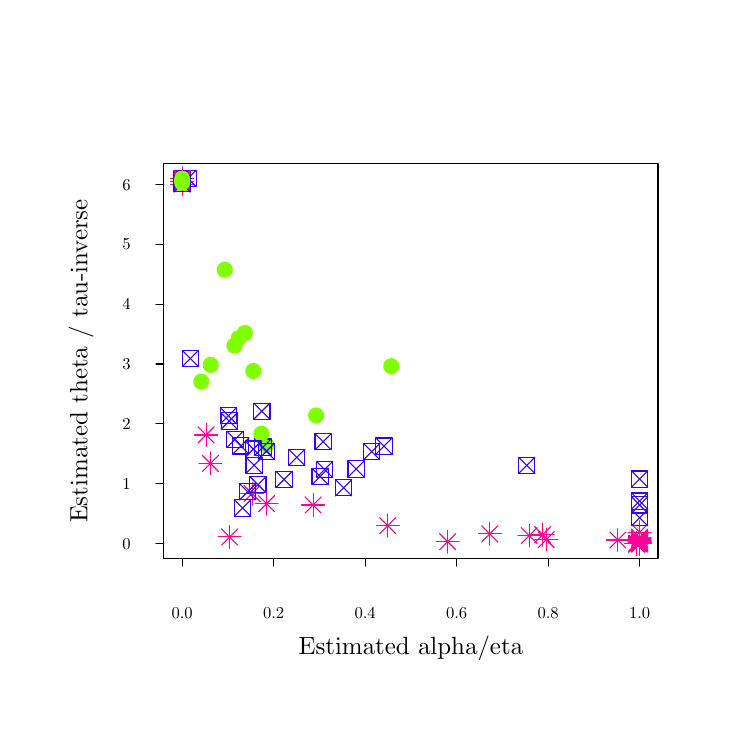
\begin{tikzpicture}[x=1pt,y=1pt]
\definecolor{fillColor}{RGB}{255,255,255}
\path[use as bounding box,fill=fillColor,fill opacity=0.00] (0,0) rectangle (252.94,252.94);
\begin{scope}
\path[clip] ( 49.20, 61.20) rectangle (227.75,203.75);
\definecolor{drawColor}{RGB}{255,0,153}

\path[draw=drawColor,line width= 0.4pt,line join=round,line cap=round] (218.21, 67.70) -- (224.06, 73.55);

\path[draw=drawColor,line width= 0.4pt,line join=round,line cap=round] (218.21, 73.55) -- (224.06, 67.70);

\path[draw=drawColor,line width= 0.4pt,line join=round,line cap=round] (216.99, 70.63) -- (225.27, 70.63);

\path[draw=drawColor,line width= 0.4pt,line join=round,line cap=round] (221.13, 66.49) -- (221.13, 74.77);

\path[draw=drawColor,line width= 0.4pt,line join=round,line cap=round] (218.21, 64.53) -- (224.06, 70.38);

\path[draw=drawColor,line width= 0.4pt,line join=round,line cap=round] (218.21, 70.38) -- (224.06, 64.53);

\path[draw=drawColor,line width= 0.4pt,line join=round,line cap=round] (217.00, 67.46) -- (225.27, 67.46);

\path[draw=drawColor,line width= 0.4pt,line join=round,line cap=round] (221.13, 63.32) -- (221.13, 71.59);

\path[draw=drawColor,line width= 0.4pt,line join=round,line cap=round] (217.14, 63.55) -- (222.99, 69.40);

\path[draw=drawColor,line width= 0.4pt,line join=round,line cap=round] (217.14, 69.40) -- (222.99, 63.55);

\path[draw=drawColor,line width= 0.4pt,line join=round,line cap=round] (215.93, 66.48) -- (224.21, 66.48);

\path[draw=drawColor,line width= 0.4pt,line join=round,line cap=round] (220.07, 62.34) -- (220.07, 70.62);
\definecolor{fillColor}{RGB}{128,255,0}

\path[fill=fillColor] ( 55.81,196.36) circle (  2.92);

\path[draw=drawColor,line width= 0.4pt,line join=round,line cap=round] ( 52.89,193.48) -- ( 58.74,199.33);

\path[draw=drawColor,line width= 0.4pt,line join=round,line cap=round] ( 52.89,199.33) -- ( 58.74,193.48);

\path[draw=drawColor,line width= 0.4pt,line join=round,line cap=round] ( 51.68,196.40) -- ( 59.95,196.40);

\path[draw=drawColor,line width= 0.4pt,line join=round,line cap=round] ( 55.81,192.27) -- ( 55.81,200.54);
\definecolor{drawColor}{RGB}{51,0,255}

\path[draw=drawColor,line width= 0.4pt,line join=round,line cap=round] (218.21, 78.96) rectangle (224.06, 84.81);

\path[draw=drawColor,line width= 0.4pt,line join=round,line cap=round] (218.21, 78.96) -- (224.06, 84.81);

\path[draw=drawColor,line width= 0.4pt,line join=round,line cap=round] (218.21, 84.81) -- (224.06, 78.96);

\path[fill=fillColor] ( 55.81,197.86) circle (  2.92);

\path[fill=fillColor] ( 55.81,197.47) circle (  2.92);

\path[fill=fillColor] ( 55.81,197.08) circle (  2.92);

\path[draw=drawColor,line width= 0.4pt,line join=round,line cap=round] ( 74.10, 98.87) rectangle ( 79.95,104.72);

\path[draw=drawColor,line width= 0.4pt,line join=round,line cap=round] ( 74.10, 98.87) -- ( 79.95,104.72);

\path[draw=drawColor,line width= 0.4pt,line join=round,line cap=round] ( 74.10,104.72) -- ( 79.95, 98.87);

\path[fill=fillColor] ( 78.50,142.61) circle (  2.92);

\path[draw=drawColor,line width= 0.4pt,line join=round,line cap=round] ( 52.89,195.14) rectangle ( 58.74,200.99);

\path[draw=drawColor,line width= 0.4pt,line join=round,line cap=round] ( 52.89,195.14) -- ( 58.74,200.99);

\path[draw=drawColor,line width= 0.4pt,line join=round,line cap=round] ( 52.89,200.99) -- ( 58.74,195.14);

\path[draw=drawColor,line width= 0.4pt,line join=round,line cap=round] (218.21, 86.91) rectangle (224.06, 92.76);

\path[draw=drawColor,line width= 0.4pt,line join=round,line cap=round] (218.21, 86.91) -- (224.06, 92.76);

\path[draw=drawColor,line width= 0.4pt,line join=round,line cap=round] (218.21, 92.76) -- (224.06, 86.91);
\definecolor{drawColor}{RGB}{255,0,153}

\path[draw=drawColor,line width= 0.4pt,line join=round,line cap=round] (184.42, 65.01) -- (190.27, 70.86);

\path[draw=drawColor,line width= 0.4pt,line join=round,line cap=round] (184.42, 70.86) -- (190.27, 65.01);

\path[draw=drawColor,line width= 0.4pt,line join=round,line cap=round] (183.21, 67.94) -- (191.49, 67.94);

\path[draw=drawColor,line width= 0.4pt,line join=round,line cap=round] (187.35, 63.80) -- (187.35, 72.07);
\definecolor{drawColor}{RGB}{51,0,255}

\path[draw=drawColor,line width= 0.4pt,line join=round,line cap=round] ( 81.70,111.44) rectangle ( 87.55,117.29);

\path[draw=drawColor,line width= 0.4pt,line join=round,line cap=round] ( 81.70,111.44) -- ( 87.55,117.29);

\path[draw=drawColor,line width= 0.4pt,line join=round,line cap=round] ( 81.70,117.29) -- ( 87.55,111.44);

\path[draw=drawColor,line width= 0.4pt,line join=round,line cap=round] (103.84,100.41) rectangle (109.69,106.26);

\path[draw=drawColor,line width= 0.4pt,line join=round,line cap=round] (103.84,100.41) -- (109.69,106.26);

\path[draw=drawColor,line width= 0.4pt,line join=round,line cap=round] (103.84,106.26) -- (109.69,100.41);

\path[draw=drawColor,line width= 0.4pt,line join=round,line cap=round] (104.36, 90.35) rectangle (110.21, 96.20);

\path[draw=drawColor,line width= 0.4pt,line join=round,line cap=round] (104.36, 90.35) -- (110.21, 96.20);

\path[draw=drawColor,line width= 0.4pt,line join=round,line cap=round] (104.36, 96.20) -- (110.21, 90.35);

\path[fill=fillColor] ( 55.81,196.52) circle (  2.92);

\path[fill=fillColor] ( 86.26,102.07) circle (  2.92);
\definecolor{drawColor}{RGB}{255,0,153}

\path[draw=drawColor,line width= 0.4pt,line join=round,line cap=round] (218.21, 64.28) -- (224.06, 70.13);

\path[draw=drawColor,line width= 0.4pt,line join=round,line cap=round] (218.21, 70.13) -- (224.06, 64.28);

\path[draw=drawColor,line width= 0.4pt,line join=round,line cap=round] (217.00, 67.20) -- (225.27, 67.20);

\path[draw=drawColor,line width= 0.4pt,line join=round,line cap=round] (221.13, 63.07) -- (221.13, 71.34);

\path[draw=drawColor,line width= 0.4pt,line join=round,line cap=round] (218.09, 63.55) -- (223.94, 69.40);

\path[draw=drawColor,line width= 0.4pt,line join=round,line cap=round] (218.09, 69.40) -- (223.94, 63.55);

\path[draw=drawColor,line width= 0.4pt,line join=round,line cap=round] (216.88, 66.48) -- (225.15, 66.48);

\path[draw=drawColor,line width= 0.4pt,line join=round,line cap=round] (221.01, 62.34) -- (221.01, 70.62);
\definecolor{drawColor}{RGB}{51,0,255}

\path[draw=drawColor,line width= 0.4pt,line join=round,line cap=round] ( 89.70, 86.76) rectangle ( 95.55, 92.61);

\path[draw=drawColor,line width= 0.4pt,line join=round,line cap=round] ( 89.70, 86.76) -- ( 95.55, 92.61);

\path[draw=drawColor,line width= 0.4pt,line join=round,line cap=round] ( 89.70, 92.61) -- ( 95.55, 86.76);
\definecolor{drawColor}{RGB}{255,0,153}

\path[draw=drawColor,line width= 0.4pt,line join=round,line cap=round] (148.84, 64.28) -- (154.69, 70.13);

\path[draw=drawColor,line width= 0.4pt,line join=round,line cap=round] (148.84, 70.13) -- (154.69, 64.28);

\path[draw=drawColor,line width= 0.4pt,line join=round,line cap=round] (147.63, 67.21) -- (155.90, 67.21);

\path[draw=drawColor,line width= 0.4pt,line join=round,line cap=round] (151.76, 63.07) -- (151.76, 71.34);

\path[draw=drawColor,line width= 0.4pt,line join=round,line cap=round] ( 52.89,194.35) -- ( 58.74,200.20);

\path[draw=drawColor,line width= 0.4pt,line join=round,line cap=round] ( 52.89,200.20) -- ( 58.74,194.35);

\path[draw=drawColor,line width= 0.4pt,line join=round,line cap=round] ( 51.68,197.28) -- ( 59.95,197.28);

\path[draw=drawColor,line width= 0.4pt,line join=round,line cap=round] ( 55.81,193.14) -- ( 55.81,201.41);

\path[draw=drawColor,line width= 0.4pt,line join=round,line cap=round] (218.09, 63.55) -- (223.94, 69.40);

\path[draw=drawColor,line width= 0.4pt,line join=round,line cap=round] (218.09, 69.40) -- (223.94, 63.55);

\path[draw=drawColor,line width= 0.4pt,line join=round,line cap=round] (216.88, 66.48) -- (225.15, 66.48);

\path[draw=drawColor,line width= 0.4pt,line join=round,line cap=round] (221.01, 62.34) -- (221.01, 70.62);

\path[fill=fillColor] (131.39,130.60) circle (  2.92);

\path[fill=fillColor] ( 62.76,125.04) circle (  2.92);

\path[draw=drawColor,line width= 0.4pt,line join=round,line cap=round] (217.14, 63.55) -- (222.99, 69.40);

\path[draw=drawColor,line width= 0.4pt,line join=round,line cap=round] (217.14, 69.40) -- (222.99, 63.55);

\path[draw=drawColor,line width= 0.4pt,line join=round,line cap=round] (215.93, 66.48) -- (224.21, 66.48);

\path[draw=drawColor,line width= 0.4pt,line join=round,line cap=round] (220.07, 62.34) -- (220.07, 70.62);

\path[draw=drawColor,line width= 0.4pt,line join=round,line cap=round] (100.20, 77.54) -- (106.05, 83.39);

\path[draw=drawColor,line width= 0.4pt,line join=round,line cap=round] (100.20, 83.39) -- (106.05, 77.54);

\path[draw=drawColor,line width= 0.4pt,line join=round,line cap=round] ( 98.99, 80.47) -- (107.27, 80.47);

\path[draw=drawColor,line width= 0.4pt,line join=round,line cap=round] (103.13, 76.33) -- (103.13, 84.60);
\definecolor{drawColor}{RGB}{51,0,255}

\path[draw=drawColor,line width= 0.4pt,line join=round,line cap=round] ( 83.30, 96.87) rectangle ( 89.15,102.72);

\path[draw=drawColor,line width= 0.4pt,line join=round,line cap=round] ( 83.30, 96.87) -- ( 89.15,102.72);

\path[draw=drawColor,line width= 0.4pt,line join=round,line cap=round] ( 83.30,102.72) -- ( 89.15, 96.87);
\definecolor{drawColor}{RGB}{255,0,153}

\path[draw=drawColor,line width= 0.4pt,line join=round,line cap=round] (218.09, 63.55) -- (223.94, 69.40);

\path[draw=drawColor,line width= 0.4pt,line join=round,line cap=round] (218.09, 69.40) -- (223.94, 63.55);

\path[draw=drawColor,line width= 0.4pt,line join=round,line cap=round] (216.88, 66.48) -- (225.15, 66.48);

\path[draw=drawColor,line width= 0.4pt,line join=round,line cap=round] (221.01, 62.34) -- (221.01, 70.62);
\definecolor{drawColor}{RGB}{51,0,255}

\path[draw=drawColor,line width= 0.4pt,line join=round,line cap=round] ( 94.31, 94.76) rectangle (100.16,100.61);

\path[draw=drawColor,line width= 0.4pt,line join=round,line cap=round] ( 94.31, 94.76) -- (100.16,100.61);

\path[draw=drawColor,line width= 0.4pt,line join=round,line cap=round] ( 94.31,100.61) -- (100.16, 94.76);

\path[draw=drawColor,line width= 0.4pt,line join=round,line cap=round] ( 69.59,109.77) rectangle ( 75.44,115.62);

\path[draw=drawColor,line width= 0.4pt,line join=round,line cap=round] ( 69.59,109.77) -- ( 75.44,115.62);

\path[draw=drawColor,line width= 0.4pt,line join=round,line cap=round] ( 69.59,115.62) -- ( 75.44,109.77);
\definecolor{drawColor}{RGB}{255,0,153}

\path[draw=drawColor,line width= 0.4pt,line join=round,line cap=round] ( 52.89,194.28) -- ( 58.74,200.13);

\path[draw=drawColor,line width= 0.4pt,line join=round,line cap=round] ( 52.89,200.13) -- ( 58.74,194.28);

\path[draw=drawColor,line width= 0.4pt,line join=round,line cap=round] ( 51.68,197.20) -- ( 59.95,197.20);

\path[draw=drawColor,line width= 0.4pt,line join=round,line cap=round] ( 55.81,193.07) -- ( 55.81,201.34);

\path[draw=drawColor,line width= 0.4pt,line join=round,line cap=round] (218.21, 63.55) -- (224.06, 69.40);

\path[draw=drawColor,line width= 0.4pt,line join=round,line cap=round] (218.21, 69.40) -- (224.06, 63.55);

\path[draw=drawColor,line width= 0.4pt,line join=round,line cap=round] (217.00, 66.48) -- (225.27, 66.48);

\path[draw=drawColor,line width= 0.4pt,line join=round,line cap=round] (221.13, 62.34) -- (221.13, 70.62);
\definecolor{drawColor}{RGB}{51,0,255}

\path[draw=drawColor,line width= 0.4pt,line join=round,line cap=round] ( 55.00,195.52) rectangle ( 60.85,201.37);

\path[draw=drawColor,line width= 0.4pt,line join=round,line cap=round] ( 55.00,195.52) -- ( 60.85,201.37);

\path[draw=drawColor,line width= 0.4pt,line join=round,line cap=round] ( 55.00,201.37) -- ( 60.85,195.52);

\path[draw=drawColor,line width= 0.4pt,line join=round,line cap=round] ( 82.10, 98.45) rectangle ( 87.95,104.30);

\path[draw=drawColor,line width= 0.4pt,line join=round,line cap=round] ( 82.10, 98.45) -- ( 87.95,104.30);

\path[draw=drawColor,line width= 0.4pt,line join=round,line cap=round] ( 82.10,104.30) -- ( 87.95, 98.45);

\path[fill=fillColor] ( 55.81,197.24) circle (  2.92);
\definecolor{drawColor}{RGB}{255,0,153}

\path[draw=drawColor,line width= 0.4pt,line join=round,line cap=round] ( 63.12, 92.55) -- ( 68.97, 98.40);

\path[draw=drawColor,line width= 0.4pt,line join=round,line cap=round] ( 63.12, 98.40) -- ( 68.97, 92.55);

\path[draw=drawColor,line width= 0.4pt,line join=round,line cap=round] ( 61.91, 95.47) -- ( 70.18, 95.47);

\path[draw=drawColor,line width= 0.4pt,line join=round,line cap=round] ( 66.04, 91.34) -- ( 66.04, 99.61);
\definecolor{drawColor}{RGB}{51,0,255}

\path[draw=drawColor,line width= 0.4pt,line join=round,line cap=round] (102.75, 87.84) rectangle (108.60, 93.69);

\path[draw=drawColor,line width= 0.4pt,line join=round,line cap=round] (102.75, 87.84) -- (108.60, 93.69);

\path[draw=drawColor,line width= 0.4pt,line join=round,line cap=round] (102.75, 93.69) -- (108.60, 87.84);

\path[fill=fillColor] ( 55.81,196.40) circle (  2.92);
\definecolor{drawColor}{RGB}{255,0,153}

\path[draw=drawColor,line width= 0.4pt,line join=round,line cap=round] (217.14, 63.55) -- (222.99, 69.40);

\path[draw=drawColor,line width= 0.4pt,line join=round,line cap=round] (217.14, 69.40) -- (222.99, 63.55);

\path[draw=drawColor,line width= 0.4pt,line join=round,line cap=round] (215.93, 66.48) -- (224.21, 66.48);

\path[draw=drawColor,line width= 0.4pt,line join=round,line cap=round] (220.07, 62.34) -- (220.07, 70.62);

\path[fill=fillColor] ( 76.29,140.79) circle (  2.92);

\path[draw=drawColor,line width= 0.4pt,line join=round,line cap=round] ( 61.54,102.85) -- ( 67.39,108.70);

\path[draw=drawColor,line width= 0.4pt,line join=round,line cap=round] ( 61.54,108.70) -- ( 67.39,102.85);

\path[draw=drawColor,line width= 0.4pt,line join=round,line cap=round] ( 60.33,105.77) -- ( 68.60,105.77);

\path[draw=drawColor,line width= 0.4pt,line join=round,line cap=round] ( 64.47,101.64) -- ( 64.47,109.91);

\path[draw=drawColor,line width= 0.4pt,line join=round,line cap=round] (217.14, 63.55) -- (222.99, 69.40);

\path[draw=drawColor,line width= 0.4pt,line join=round,line cap=round] (217.14, 69.40) -- (222.99, 63.55);

\path[draw=drawColor,line width= 0.4pt,line join=round,line cap=round] (215.93, 66.48) -- (224.21, 66.48);

\path[draw=drawColor,line width= 0.4pt,line join=round,line cap=round] (220.07, 62.34) -- (220.07, 70.62);
\definecolor{drawColor}{RGB}{51,0,255}

\path[draw=drawColor,line width= 0.4pt,line join=round,line cap=round] (111.26, 83.75) rectangle (117.11, 89.60);

\path[draw=drawColor,line width= 0.4pt,line join=round,line cap=round] (111.26, 83.75) -- (117.11, 89.60);

\path[draw=drawColor,line width= 0.4pt,line join=round,line cap=round] (111.26, 89.60) -- (117.11, 83.75);

\path[draw=drawColor,line width= 0.4pt,line join=round,line cap=round] ( 74.74, 76.46) rectangle ( 80.59, 82.31);

\path[draw=drawColor,line width= 0.4pt,line join=round,line cap=round] ( 74.74, 76.46) -- ( 80.59, 82.31);

\path[draw=drawColor,line width= 0.4pt,line join=round,line cap=round] ( 74.74, 82.31) -- ( 80.59, 76.46);

\path[fill=fillColor] ( 55.81,198.24) circle (  2.92);
\definecolor{drawColor}{RGB}{255,0,153}

\path[draw=drawColor,line width= 0.4pt,line join=round,line cap=round] (217.14, 63.55) -- (222.99, 69.40);

\path[draw=drawColor,line width= 0.4pt,line join=round,line cap=round] (217.14, 69.40) -- (222.99, 63.55);

\path[draw=drawColor,line width= 0.4pt,line join=round,line cap=round] (215.93, 66.48) -- (224.21, 66.48);

\path[draw=drawColor,line width= 0.4pt,line join=round,line cap=round] (220.07, 62.34) -- (220.07, 70.62);

\path[fill=fillColor] ( 55.81,197.55) circle (  2.92);

\path[fill=fillColor] ( 66.14,131.07) circle (  2.92);

\path[draw=drawColor,line width= 0.4pt,line join=round,line cap=round] ( 78.17, 81.66) -- ( 84.02, 87.51);

\path[draw=drawColor,line width= 0.4pt,line join=round,line cap=round] ( 78.17, 87.51) -- ( 84.02, 81.66);

\path[draw=drawColor,line width= 0.4pt,line join=round,line cap=round] ( 76.96, 84.59) -- ( 85.23, 84.59);

\path[draw=drawColor,line width= 0.4pt,line join=round,line cap=round] ( 81.10, 80.45) -- ( 81.10, 88.72);
\definecolor{drawColor}{RGB}{51,0,255}

\path[draw=drawColor,line width= 0.4pt,line join=round,line cap=round] ( 52.89,195.54) rectangle ( 58.74,201.39);

\path[draw=drawColor,line width= 0.4pt,line join=round,line cap=round] ( 52.89,195.54) -- ( 58.74,201.39);

\path[draw=drawColor,line width= 0.4pt,line join=round,line cap=round] ( 52.89,201.39) -- ( 58.74,195.54);
\definecolor{drawColor}{RGB}{255,0,153}

\path[draw=drawColor,line width= 0.4pt,line join=round,line cap=round] (178.32, 66.48) -- (184.17, 72.33);

\path[draw=drawColor,line width= 0.4pt,line join=round,line cap=round] (178.32, 72.33) -- (184.17, 66.48);

\path[draw=drawColor,line width= 0.4pt,line join=round,line cap=round] (177.11, 69.41) -- (185.38, 69.41);

\path[draw=drawColor,line width= 0.4pt,line join=round,line cap=round] (181.25, 65.27) -- (181.25, 73.54);

\path[fill=fillColor] ( 81.52,128.87) circle (  2.92);

\path[fill=fillColor] ( 71.21,165.47) circle (  2.92);

\path[draw=drawColor,line width= 0.4pt,line join=round,line cap=round] ( 52.89,194.34) -- ( 58.74,200.19);

\path[draw=drawColor,line width= 0.4pt,line join=round,line cap=round] ( 52.89,200.19) -- ( 58.74,194.34);

\path[draw=drawColor,line width= 0.4pt,line join=round,line cap=round] ( 51.68,197.27) -- ( 59.95,197.27);

\path[draw=drawColor,line width= 0.4pt,line join=round,line cap=round] ( 55.81,193.13) -- ( 55.81,201.40);

\path[draw=drawColor,line width= 0.4pt,line join=round,line cap=round] ( 52.89,195.48) -- ( 58.74,201.33);

\path[draw=drawColor,line width= 0.4pt,line join=round,line cap=round] ( 52.89,201.33) -- ( 58.74,195.48);

\path[draw=drawColor,line width= 0.4pt,line join=round,line cap=round] ( 51.68,198.41) -- ( 59.95,198.41);

\path[draw=drawColor,line width= 0.4pt,line join=round,line cap=round] ( 55.81,194.27) -- ( 55.81,202.55);
\definecolor{drawColor}{RGB}{51,0,255}

\path[draw=drawColor,line width= 0.4pt,line join=round,line cap=round] (218.21, 77.56) rectangle (224.06, 83.41);

\path[draw=drawColor,line width= 0.4pt,line join=round,line cap=round] (218.21, 77.56) -- (224.06, 83.41);

\path[draw=drawColor,line width= 0.4pt,line join=round,line cap=round] (218.21, 83.41) -- (224.06, 77.56);

\path[draw=drawColor,line width= 0.4pt,line join=round,line cap=round] ( 76.56, 82.29) rectangle ( 82.41, 88.14);

\path[draw=drawColor,line width= 0.4pt,line join=round,line cap=round] ( 76.56, 82.29) -- ( 82.41, 88.14);

\path[draw=drawColor,line width= 0.4pt,line join=round,line cap=round] ( 76.56, 88.14) -- ( 82.41, 82.29);
\definecolor{drawColor}{RGB}{255,0,153}

\path[draw=drawColor,line width= 0.4pt,line join=round,line cap=round] (218.21, 64.13) -- (224.06, 69.98);

\path[draw=drawColor,line width= 0.4pt,line join=round,line cap=round] (218.21, 69.98) -- (224.06, 64.13);

\path[draw=drawColor,line width= 0.4pt,line join=round,line cap=round] (217.00, 67.06) -- (225.27, 67.06);

\path[draw=drawColor,line width= 0.4pt,line join=round,line cap=round] (221.13, 62.92) -- (221.13, 71.19);
\definecolor{drawColor}{RGB}{51,0,255}

\path[draw=drawColor,line width= 0.4pt,line join=round,line cap=round] ( 71.99,101.26) rectangle ( 77.84,107.11);

\path[draw=drawColor,line width= 0.4pt,line join=round,line cap=round] ( 71.99,101.26) -- ( 77.84,107.11);

\path[draw=drawColor,line width= 0.4pt,line join=round,line cap=round] ( 71.99,107.11) -- ( 77.84,101.26);
\definecolor{drawColor}{RGB}{255,0,153}

\path[draw=drawColor,line width= 0.4pt,line join=round,line cap=round] (218.21, 63.55) -- (224.06, 69.40);

\path[draw=drawColor,line width= 0.4pt,line join=round,line cap=round] (218.21, 69.40) -- (224.06, 63.55);

\path[draw=drawColor,line width= 0.4pt,line join=round,line cap=round] (217.00, 66.48) -- (225.27, 66.48);

\path[draw=drawColor,line width= 0.4pt,line join=round,line cap=round] (221.13, 62.34) -- (221.13, 70.62);

\path[draw=drawColor,line width= 0.4pt,line join=round,line cap=round] ( 70.05, 65.99) -- ( 75.90, 71.84);

\path[draw=drawColor,line width= 0.4pt,line join=round,line cap=round] ( 70.05, 71.84) -- ( 75.90, 65.99);

\path[draw=drawColor,line width= 0.4pt,line join=round,line cap=round] ( 68.84, 68.92) -- ( 77.11, 68.92);

\path[draw=drawColor,line width= 0.4pt,line join=round,line cap=round] ( 72.98, 64.78) -- ( 72.98, 73.05);
\definecolor{drawColor}{RGB}{51,0,255}

\path[draw=drawColor,line width= 0.4pt,line join=round,line cap=round] ( 55.87,130.47) rectangle ( 61.72,136.32);

\path[draw=drawColor,line width= 0.4pt,line join=round,line cap=round] ( 55.87,130.47) -- ( 61.72,136.32);

\path[draw=drawColor,line width= 0.4pt,line join=round,line cap=round] ( 55.87,136.32) -- ( 61.72,130.47);
\definecolor{drawColor}{RGB}{255,0,153}

\path[draw=drawColor,line width= 0.4pt,line join=round,line cap=round] (218.21, 65.12) -- (224.06, 70.97);

\path[draw=drawColor,line width= 0.4pt,line join=round,line cap=round] (218.21, 70.97) -- (224.06, 65.12);

\path[draw=drawColor,line width= 0.4pt,line join=round,line cap=round] (217.00, 68.05) -- (225.27, 68.05);

\path[draw=drawColor,line width= 0.4pt,line join=round,line cap=round] (221.13, 63.91) -- (221.13, 72.18);

\path[draw=drawColor,line width= 0.4pt,line join=round,line cap=round] ( 52.89,195.42) -- ( 58.74,201.27);

\path[draw=drawColor,line width= 0.4pt,line join=round,line cap=round] ( 52.89,201.27) -- ( 58.74,195.42);

\path[draw=drawColor,line width= 0.4pt,line join=round,line cap=round] ( 51.68,198.35) -- ( 59.95,198.35);

\path[draw=drawColor,line width= 0.4pt,line join=round,line cap=round] ( 55.81,194.21) -- ( 55.81,202.48);

\path[fill=fillColor] ( 84.46,106.19) circle (  2.92);
\definecolor{drawColor}{RGB}{51,0,255}

\path[draw=drawColor,line width= 0.4pt,line join=round,line cap=round] ( 80.27, 84.89) rectangle ( 86.12, 90.74);

\path[draw=drawColor,line width= 0.4pt,line join=round,line cap=round] ( 80.27, 84.89) -- ( 86.12, 90.74);

\path[draw=drawColor,line width= 0.4pt,line join=round,line cap=round] ( 80.27, 90.74) -- ( 86.12, 84.89);
\definecolor{drawColor}{RGB}{255,0,153}

\path[draw=drawColor,line width= 0.4pt,line join=round,line cap=round] (127.20, 70.09) -- (133.05, 75.94);

\path[draw=drawColor,line width= 0.4pt,line join=round,line cap=round] (127.20, 75.94) -- (133.05, 70.09);

\path[draw=drawColor,line width= 0.4pt,line join=round,line cap=round] (125.99, 73.01) -- (134.26, 73.01);

\path[draw=drawColor,line width= 0.4pt,line join=round,line cap=round] (130.13, 68.88) -- (130.13, 77.15);

\path[draw=drawColor,line width= 0.4pt,line join=round,line cap=round] ( 83.40, 78.00) -- ( 89.25, 83.85);

\path[draw=drawColor,line width= 0.4pt,line join=round,line cap=round] ( 83.40, 83.85) -- ( 89.25, 78.00);

\path[draw=drawColor,line width= 0.4pt,line join=round,line cap=round] ( 82.18, 80.93) -- ( 90.46, 80.93);

\path[draw=drawColor,line width= 0.4pt,line join=round,line cap=round] ( 86.32, 76.79) -- ( 86.32, 85.06);

\path[draw=drawColor,line width= 0.4pt,line join=round,line cap=round] (217.14, 63.55) -- (222.99, 69.40);

\path[draw=drawColor,line width= 0.4pt,line join=round,line cap=round] (217.14, 69.40) -- (222.99, 63.55);

\path[draw=drawColor,line width= 0.4pt,line join=round,line cap=round] (215.93, 66.48) -- (224.21, 66.48);

\path[draw=drawColor,line width= 0.4pt,line join=round,line cap=round] (220.07, 62.34) -- (220.07, 70.62);

\path[draw=drawColor,line width= 0.4pt,line join=round,line cap=round] ( 52.89,195.45) -- ( 58.74,201.30);

\path[draw=drawColor,line width= 0.4pt,line join=round,line cap=round] ( 52.89,201.30) -- ( 58.74,195.45);

\path[draw=drawColor,line width= 0.4pt,line join=round,line cap=round] ( 51.68,198.37) -- ( 59.95,198.37);

\path[draw=drawColor,line width= 0.4pt,line join=round,line cap=round] ( 55.81,194.23) -- ( 55.81,202.51);

\path[draw=drawColor,line width= 0.4pt,line join=round,line cap=round] ( 52.89,194.59) -- ( 58.74,200.44);

\path[draw=drawColor,line width= 0.4pt,line join=round,line cap=round] ( 52.89,200.44) -- ( 58.74,194.59);

\path[draw=drawColor,line width= 0.4pt,line join=round,line cap=round] ( 51.68,197.51) -- ( 59.95,197.51);

\path[draw=drawColor,line width= 0.4pt,line join=round,line cap=round] ( 55.81,193.38) -- ( 55.81,201.65);
\definecolor{drawColor}{RGB}{51,0,255}

\path[draw=drawColor,line width= 0.4pt,line join=round,line cap=round] ( 78.91, 91.91) rectangle ( 84.76, 97.76);

\path[draw=drawColor,line width= 0.4pt,line join=round,line cap=round] ( 78.91, 91.91) -- ( 84.76, 97.76);

\path[draw=drawColor,line width= 0.4pt,line join=round,line cap=round] ( 78.91, 97.76) -- ( 84.76, 91.91);

\path[fill=fillColor] ( 55.81,198.37) circle (  2.92);

\path[draw=drawColor,line width= 0.4pt,line join=round,line cap=round] ( 52.89,193.73) rectangle ( 58.74,199.58);

\path[draw=drawColor,line width= 0.4pt,line join=round,line cap=round] ( 52.89,193.73) -- ( 58.74,199.58);

\path[draw=drawColor,line width= 0.4pt,line join=round,line cap=round] ( 52.89,199.58) -- ( 58.74,193.73);
\definecolor{drawColor}{RGB}{255,0,153}

\path[draw=drawColor,line width= 0.4pt,line join=round,line cap=round] (217.14, 63.55) -- (222.99, 69.40);

\path[draw=drawColor,line width= 0.4pt,line join=round,line cap=round] (217.14, 69.40) -- (222.99, 63.55);

\path[draw=drawColor,line width= 0.4pt,line join=round,line cap=round] (215.93, 66.48) -- (224.21, 66.48);

\path[draw=drawColor,line width= 0.4pt,line join=round,line cap=round] (220.07, 62.34) -- (220.07, 70.62);

\path[draw=drawColor,line width= 0.4pt,line join=round,line cap=round] (217.14, 63.55) -- (222.99, 69.40);

\path[draw=drawColor,line width= 0.4pt,line join=round,line cap=round] (217.14, 69.40) -- (222.99, 63.55);

\path[draw=drawColor,line width= 0.4pt,line join=round,line cap=round] (215.93, 66.48) -- (224.21, 66.48);

\path[draw=drawColor,line width= 0.4pt,line join=round,line cap=round] (220.07, 62.34) -- (220.07, 70.62);
\definecolor{drawColor}{RGB}{51,0,255}

\path[draw=drawColor,line width= 0.4pt,line join=round,line cap=round] (115.76, 90.55) rectangle (121.61, 96.40);

\path[draw=drawColor,line width= 0.4pt,line join=round,line cap=round] (115.76, 90.55) -- (121.61, 96.40);

\path[draw=drawColor,line width= 0.4pt,line join=round,line cap=round] (115.76, 96.40) -- (121.61, 90.55);

\path[fill=fillColor] ( 74.73,138.05) circle (  2.92);
\definecolor{drawColor}{RGB}{255,0,153}

\path[draw=drawColor,line width= 0.4pt,line join=round,line cap=round] (217.14, 63.55) -- (222.99, 69.40);

\path[draw=drawColor,line width= 0.4pt,line join=round,line cap=round] (217.14, 69.40) -- (222.99, 63.55);

\path[draw=drawColor,line width= 0.4pt,line join=round,line cap=round] (215.93, 66.48) -- (224.21, 66.48);

\path[draw=drawColor,line width= 0.4pt,line join=round,line cap=round] (220.07, 62.34) -- (220.07, 70.62);

\path[fill=fillColor] (104.23,112.82) circle (  2.92);

\path[draw=drawColor,line width= 0.4pt,line join=round,line cap=round] (218.21, 63.55) -- (224.06, 69.40);

\path[draw=drawColor,line width= 0.4pt,line join=round,line cap=round] (218.21, 69.40) -- (224.06, 63.55);

\path[draw=drawColor,line width= 0.4pt,line join=round,line cap=round] (217.00, 66.48) -- (225.27, 66.48);

\path[draw=drawColor,line width= 0.4pt,line join=round,line cap=round] (221.13, 62.34) -- (221.13, 70.62);

\path[draw=drawColor,line width= 0.4pt,line join=round,line cap=round] (217.14, 63.55) -- (222.99, 69.40);

\path[draw=drawColor,line width= 0.4pt,line join=round,line cap=round] (217.14, 69.40) -- (222.99, 63.55);

\path[draw=drawColor,line width= 0.4pt,line join=round,line cap=round] (215.93, 66.48) -- (224.21, 66.48);

\path[draw=drawColor,line width= 0.4pt,line join=round,line cap=round] (220.07, 62.34) -- (220.07, 70.62);
\definecolor{drawColor}{RGB}{51,0,255}

\path[draw=drawColor,line width= 0.4pt,line join=round,line cap=round] (121.40, 96.82) rectangle (127.25,102.67);

\path[draw=drawColor,line width= 0.4pt,line join=round,line cap=round] (121.40, 96.82) -- (127.25,102.67);

\path[draw=drawColor,line width= 0.4pt,line join=round,line cap=round] (121.40,102.67) -- (127.25, 96.82);
\definecolor{drawColor}{RGB}{255,0,153}

\path[draw=drawColor,line width= 0.4pt,line join=round,line cap=round] (218.21, 63.55) -- (224.06, 69.40);

\path[draw=drawColor,line width= 0.4pt,line join=round,line cap=round] (218.21, 69.40) -- (224.06, 63.55);

\path[draw=drawColor,line width= 0.4pt,line join=round,line cap=round] (217.00, 66.48) -- (225.27, 66.48);

\path[draw=drawColor,line width= 0.4pt,line join=round,line cap=round] (221.13, 62.34) -- (221.13, 70.62);

\path[fill=fillColor] ( 55.81,198.10) circle (  2.92);
\definecolor{drawColor}{RGB}{51,0,255}

\path[draw=drawColor,line width= 0.4pt,line join=round,line cap=round] ( 69.90,107.88) rectangle ( 75.75,113.73);

\path[draw=drawColor,line width= 0.4pt,line join=round,line cap=round] ( 69.90,107.88) -- ( 75.75,113.73);

\path[draw=drawColor,line width= 0.4pt,line join=round,line cap=round] ( 69.90,113.73) -- ( 75.75,107.88);
\definecolor{drawColor}{RGB}{255,0,153}

\path[draw=drawColor,line width= 0.4pt,line join=round,line cap=round] (217.14, 63.55) -- (222.99, 69.40);

\path[draw=drawColor,line width= 0.4pt,line join=round,line cap=round] (217.14, 69.40) -- (222.99, 63.55);

\path[draw=drawColor,line width= 0.4pt,line join=round,line cap=round] (215.93, 66.48) -- (224.21, 66.48);

\path[draw=drawColor,line width= 0.4pt,line join=round,line cap=round] (220.07, 62.34) -- (220.07, 70.62);

\path[draw=drawColor,line width= 0.4pt,line join=round,line cap=round] (164.06, 67.09) -- (169.91, 72.94);

\path[draw=drawColor,line width= 0.4pt,line join=round,line cap=round] (164.06, 72.94) -- (169.91, 67.09);

\path[draw=drawColor,line width= 0.4pt,line join=round,line cap=round] (162.85, 70.02) -- (171.12, 70.02);

\path[draw=drawColor,line width= 0.4pt,line join=round,line cap=round] (166.99, 65.88) -- (166.99, 74.15);
\definecolor{drawColor}{RGB}{51,0,255}

\path[draw=drawColor,line width= 0.4pt,line join=round,line cap=round] (125.84, 98.82) rectangle (131.69,104.67);

\path[draw=drawColor,line width= 0.4pt,line join=round,line cap=round] (125.84, 98.82) -- (131.69,104.67);

\path[draw=drawColor,line width= 0.4pt,line join=round,line cap=round] (125.84,104.67) -- (131.69, 98.82);

\path[draw=drawColor,line width= 0.4pt,line join=round,line cap=round] ( 78.63, 97.72) rectangle ( 84.48,103.57);

\path[draw=drawColor,line width= 0.4pt,line join=round,line cap=round] ( 78.63, 97.72) -- ( 84.48,103.57);

\path[draw=drawColor,line width= 0.4pt,line join=round,line cap=round] ( 78.63,103.57) -- ( 84.48, 97.72);
\definecolor{drawColor}{RGB}{255,0,153}

\path[draw=drawColor,line width= 0.4pt,line join=round,line cap=round] (218.21, 65.39) -- (224.06, 71.24);

\path[draw=drawColor,line width= 0.4pt,line join=round,line cap=round] (218.21, 71.24) -- (224.06, 65.39);

\path[draw=drawColor,line width= 0.4pt,line join=round,line cap=round] (217.00, 68.32) -- (225.27, 68.32);

\path[draw=drawColor,line width= 0.4pt,line join=round,line cap=round] (221.13, 64.18) -- (221.13, 72.46);

\path[draw=drawColor,line width= 0.4pt,line join=round,line cap=round] (217.14, 63.55) -- (222.99, 69.40);

\path[draw=drawColor,line width= 0.4pt,line join=round,line cap=round] (217.14, 69.40) -- (222.99, 63.55);

\path[draw=drawColor,line width= 0.4pt,line join=round,line cap=round] (215.93, 66.48) -- (224.21, 66.48);

\path[draw=drawColor,line width= 0.4pt,line join=round,line cap=round] (220.07, 62.34) -- (220.07, 70.62);
\definecolor{drawColor}{RGB}{51,0,255}

\path[draw=drawColor,line width= 0.4pt,line join=round,line cap=round] (218.21, 72.94) rectangle (224.06, 78.79);

\path[draw=drawColor,line width= 0.4pt,line join=round,line cap=round] (218.21, 72.94) -- (224.06, 78.79);

\path[draw=drawColor,line width= 0.4pt,line join=round,line cap=round] (218.21, 78.79) -- (224.06, 72.94);
\definecolor{drawColor}{RGB}{255,0,153}

\path[draw=drawColor,line width= 0.4pt,line join=round,line cap=round] (210.35, 64.88) -- (216.20, 70.73);

\path[draw=drawColor,line width= 0.4pt,line join=round,line cap=round] (210.35, 70.73) -- (216.20, 64.88);

\path[draw=drawColor,line width= 0.4pt,line join=round,line cap=round] (209.14, 67.81) -- (217.41, 67.81);

\path[draw=drawColor,line width= 0.4pt,line join=round,line cap=round] (213.27, 63.67) -- (213.27, 71.94);

\path[fill=fillColor] ( 55.81,197.65) circle (  2.92);

\path[draw=drawColor,line width= 0.4pt,line join=round,line cap=round] (218.20, 63.89) -- (224.05, 69.74);

\path[draw=drawColor,line width= 0.4pt,line join=round,line cap=round] (218.20, 69.74) -- (224.05, 63.89);

\path[draw=drawColor,line width= 0.4pt,line join=round,line cap=round] (216.99, 66.82) -- (225.26, 66.82);

\path[draw=drawColor,line width= 0.4pt,line join=round,line cap=round] (221.13, 62.68) -- (221.13, 70.95);

\path[draw=drawColor,line width= 0.4pt,line join=round,line cap=round] (217.14, 63.55) -- (222.99, 69.40);

\path[draw=drawColor,line width= 0.4pt,line join=round,line cap=round] (217.14, 69.40) -- (222.99, 63.55);

\path[draw=drawColor,line width= 0.4pt,line join=round,line cap=round] (215.93, 66.48) -- (224.21, 66.48);

\path[draw=drawColor,line width= 0.4pt,line join=round,line cap=round] (220.07, 62.34) -- (220.07, 70.62);

\path[draw=drawColor,line width= 0.4pt,line join=round,line cap=round] (218.21, 65.90) -- (224.06, 71.75);

\path[draw=drawColor,line width= 0.4pt,line join=round,line cap=round] (218.21, 71.75) -- (224.06, 65.90);

\path[draw=drawColor,line width= 0.4pt,line join=round,line cap=round] (217.00, 68.83) -- (225.27, 68.83);

\path[draw=drawColor,line width= 0.4pt,line join=round,line cap=round] (221.13, 64.69) -- (221.13, 72.97);

\path[draw=drawColor,line width= 0.4pt,line join=round,line cap=round] (183.17, 66.80) -- (189.02, 72.65);

\path[draw=drawColor,line width= 0.4pt,line join=round,line cap=round] (183.17, 72.65) -- (189.02, 66.80);

\path[draw=drawColor,line width= 0.4pt,line join=round,line cap=round] (181.96, 69.72) -- (190.23, 69.72);

\path[draw=drawColor,line width= 0.4pt,line join=round,line cap=round] (186.10, 65.59) -- (186.10, 73.86);

\path[fill=fillColor] ( 55.81,197.02) circle (  2.92);
\definecolor{drawColor}{RGB}{51,0,255}

\path[draw=drawColor,line width= 0.4pt,line join=round,line cap=round] (177.43, 91.84) rectangle (183.28, 97.69);

\path[draw=drawColor,line width= 0.4pt,line join=round,line cap=round] (177.43, 91.84) -- (183.28, 97.69);

\path[draw=drawColor,line width= 0.4pt,line join=round,line cap=round] (177.43, 97.69) -- (183.28, 91.84);
\end{scope}
\begin{scope}
\path[clip] (  0.00,  0.00) rectangle (252.94,252.94);
\definecolor{drawColor}{RGB}{0,0,0}

\path[draw=drawColor,line width= 0.4pt,line join=round,line cap=round] ( 55.81, 61.20) -- (221.13, 61.20);

\path[draw=drawColor,line width= 0.4pt,line join=round,line cap=round] ( 55.81, 61.20) -- ( 55.81, 58.35);

\path[draw=drawColor,line width= 0.4pt,line join=round,line cap=round] ( 88.88, 61.20) -- ( 88.88, 58.35);

\path[draw=drawColor,line width= 0.4pt,line join=round,line cap=round] (121.94, 61.20) -- (121.94, 58.35);

\path[draw=drawColor,line width= 0.4pt,line join=round,line cap=round] (155.00, 61.20) -- (155.00, 58.35);

\path[draw=drawColor,line width= 0.4pt,line join=round,line cap=round] (188.07, 61.20) -- (188.07, 58.35);

\path[draw=drawColor,line width= 0.4pt,line join=round,line cap=round] (221.13, 61.20) -- (221.13, 58.35);

\node[text=drawColor,anchor=base,inner sep=0pt, outer sep=0pt, scale=  0.60] at ( 55.81, 39.60) {0.0};

\node[text=drawColor,anchor=base,inner sep=0pt, outer sep=0pt, scale=  0.60] at ( 88.88, 39.60) {0.2};

\node[text=drawColor,anchor=base,inner sep=0pt, outer sep=0pt, scale=  0.60] at (121.94, 39.60) {0.4};

\node[text=drawColor,anchor=base,inner sep=0pt, outer sep=0pt, scale=  0.60] at (155.00, 39.60) {0.6};

\node[text=drawColor,anchor=base,inner sep=0pt, outer sep=0pt, scale=  0.60] at (188.07, 39.60) {0.8};

\node[text=drawColor,anchor=base,inner sep=0pt, outer sep=0pt, scale=  0.60] at (221.13, 39.60) {1.0};

\path[draw=drawColor,line width= 0.4pt,line join=round,line cap=round] ( 49.20, 66.48) -- ( 49.20,196.32);

\path[draw=drawColor,line width= 0.4pt,line join=round,line cap=round] ( 49.20, 66.48) -- ( 46.35, 66.48);

\path[draw=drawColor,line width= 0.4pt,line join=round,line cap=round] ( 49.20, 88.12) -- ( 46.35, 88.12);

\path[draw=drawColor,line width= 0.4pt,line join=round,line cap=round] ( 49.20,109.76) -- ( 46.35,109.76);

\path[draw=drawColor,line width= 0.4pt,line join=round,line cap=round] ( 49.20,131.40) -- ( 46.35,131.40);

\path[draw=drawColor,line width= 0.4pt,line join=round,line cap=round] ( 49.20,153.04) -- ( 46.35,153.04);

\path[draw=drawColor,line width= 0.4pt,line join=round,line cap=round] ( 49.20,174.68) -- ( 46.35,174.68);

\path[draw=drawColor,line width= 0.4pt,line join=round,line cap=round] ( 49.20,196.32) -- ( 46.35,196.32);

\node[text=drawColor,anchor=base east,inner sep=0pt, outer sep=0pt, scale=  0.60] at ( 37.20, 64.41) {0};

\node[text=drawColor,anchor=base east,inner sep=0pt, outer sep=0pt, scale=  0.60] at ( 37.20, 86.05) {1};

\node[text=drawColor,anchor=base east,inner sep=0pt, outer sep=0pt, scale=  0.60] at ( 37.20,107.69) {2};

\node[text=drawColor,anchor=base east,inner sep=0pt, outer sep=0pt, scale=  0.60] at ( 37.20,129.33) {3};

\node[text=drawColor,anchor=base east,inner sep=0pt, outer sep=0pt, scale=  0.60] at ( 37.20,150.97) {4};

\node[text=drawColor,anchor=base east,inner sep=0pt, outer sep=0pt, scale=  0.60] at ( 37.20,172.61) {5};

\node[text=drawColor,anchor=base east,inner sep=0pt, outer sep=0pt, scale=  0.60] at ( 37.20,194.25) {6};

\path[draw=drawColor,line width= 0.4pt,line join=round,line cap=round] ( 49.20, 61.20) --
	(227.75, 61.20) --
	(227.75,203.75) --
	( 49.20,203.75) --
	( 49.20, 61.20);
\end{scope}
\begin{scope}
\path[clip] (  0.00,  0.00) rectangle (252.94,252.94);
\definecolor{drawColor}{RGB}{0,0,0}

\node[text=drawColor,anchor=base,inner sep=0pt, outer sep=0pt, scale=  0.90] at (138.47, 26.40) {Estimated alpha/eta};

\node[text=drawColor,rotate= 90.00,anchor=base,inner sep=0pt, outer sep=0pt, scale=  0.90] at ( 21.60,132.47) {Estimated theta / tau-inverse};
\end{scope}
\end{tikzpicture}

\end{frame}
	
\begin{frame}{Experiment Results}
	\framesubtitle{Multi arm bandit experiments - 2 Clusters / Spectral RBF / Blockwise Entropy}
	\center
	 % Created by tikzDevice version 0.10.1 on 2016-06-30 12:40:44
% !TEX encoding = UTF-8 Unicode
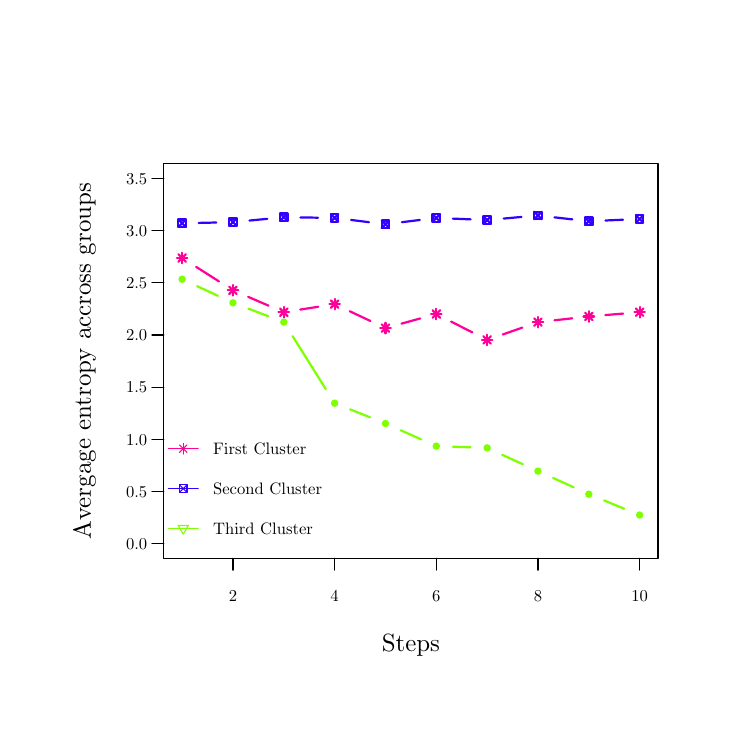
\begin{tikzpicture}[x=1pt,y=1pt]
\definecolor{fillColor}{RGB}{255,255,255}
\path[use as bounding box,fill=fillColor,fill opacity=0.00] (0,0) rectangle (252.94,252.94);
\begin{scope}
\path[clip] ( 49.20, 61.20) rectangle (227.75,203.75);
\definecolor{drawColor}{RGB}{255,0,153}

\path[draw=drawColor,line width= 0.8pt,line join=round,line cap=round] ( 60.88,166.49) -- ( 69.12,161.26);

\path[draw=drawColor,line width= 0.8pt,line join=round,line cap=round] ( 79.69,155.66) -- ( 87.04,152.49);

\path[draw=drawColor,line width= 0.8pt,line join=round,line cap=round] ( 98.48,151.06) -- (104.99,152.09);

\path[draw=drawColor,line width= 0.8pt,line join=round,line cap=round] (116.35,150.48) -- (123.86,146.94);

\path[draw=drawColor,line width= 0.8pt,line join=round,line cap=round] (135.07,145.98) -- (141.87,147.87);

\path[draw=drawColor,line width= 0.8pt,line join=round,line cap=round] (153.00,146.74) -- (160.68,142.82);

\path[draw=drawColor,line width= 0.8pt,line join=round,line cap=round] (171.69,142.08) -- (178.73,144.55);

\path[draw=drawColor,line width= 0.8pt,line join=round,line cap=round] (190.36,147.20) -- (196.80,147.92);

\path[draw=drawColor,line width= 0.8pt,line join=round,line cap=round] (208.74,149.09) -- (215.15,149.62);

\path[draw=drawColor,line width= 0.8pt,line join=round,line cap=round] ( 54.46,168.36) -- ( 57.16,171.06);

\path[draw=drawColor,line width= 0.8pt,line join=round,line cap=round] ( 54.46,171.06) -- ( 57.16,168.36);

\path[draw=drawColor,line width= 0.8pt,line join=round,line cap=round] ( 53.90,169.71) -- ( 57.72,169.71);

\path[draw=drawColor,line width= 0.8pt,line join=round,line cap=round] ( 55.81,167.80) -- ( 55.81,171.62);

\path[draw=drawColor,line width= 0.8pt,line join=round,line cap=round] ( 72.83,156.69) -- ( 75.53,159.39);

\path[draw=drawColor,line width= 0.8pt,line join=round,line cap=round] ( 72.83,159.39) -- ( 75.53,156.69);

\path[draw=drawColor,line width= 0.8pt,line join=round,line cap=round] ( 72.27,158.04) -- ( 76.09,158.04);

\path[draw=drawColor,line width= 0.8pt,line join=round,line cap=round] ( 74.18,156.13) -- ( 74.18,159.95);

\path[draw=drawColor,line width= 0.8pt,line join=round,line cap=round] ( 91.20,148.76) -- ( 93.90,151.46);

\path[draw=drawColor,line width= 0.8pt,line join=round,line cap=round] ( 91.20,151.46) -- ( 93.90,148.76);

\path[draw=drawColor,line width= 0.8pt,line join=round,line cap=round] ( 90.64,150.11) -- ( 94.46,150.11);

\path[draw=drawColor,line width= 0.8pt,line join=round,line cap=round] ( 92.55,148.20) -- ( 92.55,152.02);

\path[draw=drawColor,line width= 0.8pt,line join=round,line cap=round] (109.57,151.69) -- (112.27,154.39);

\path[draw=drawColor,line width= 0.8pt,line join=round,line cap=round] (109.57,154.39) -- (112.27,151.69);

\path[draw=drawColor,line width= 0.8pt,line join=round,line cap=round] (109.01,153.04) -- (112.83,153.04);

\path[draw=drawColor,line width= 0.8pt,line join=round,line cap=round] (110.92,151.13) -- (110.92,154.95);

\path[draw=drawColor,line width= 0.8pt,line join=round,line cap=round] (127.94,143.03) -- (130.64,145.73);

\path[draw=drawColor,line width= 0.8pt,line join=round,line cap=round] (127.94,145.73) -- (130.64,143.03);

\path[draw=drawColor,line width= 0.8pt,line join=round,line cap=round] (127.38,144.38) -- (131.20,144.38);

\path[draw=drawColor,line width= 0.8pt,line join=round,line cap=round] (129.29,142.47) -- (129.29,146.29);

\path[draw=drawColor,line width= 0.8pt,line join=round,line cap=round] (146.31,148.12) -- (149.01,150.82);

\path[draw=drawColor,line width= 0.8pt,line join=round,line cap=round] (146.31,150.82) -- (149.01,148.12);

\path[draw=drawColor,line width= 0.8pt,line join=round,line cap=round] (145.75,149.47) -- (149.57,149.47);

\path[draw=drawColor,line width= 0.8pt,line join=round,line cap=round] (147.66,147.56) -- (147.66,151.38);

\path[draw=drawColor,line width= 0.8pt,line join=round,line cap=round] (164.68,138.74) -- (167.38,141.44);

\path[draw=drawColor,line width= 0.8pt,line join=round,line cap=round] (164.68,141.44) -- (167.38,138.74);

\path[draw=drawColor,line width= 0.8pt,line join=round,line cap=round] (164.12,140.09) -- (167.93,140.09);

\path[draw=drawColor,line width= 0.8pt,line join=round,line cap=round] (166.03,138.18) -- (166.03,142.00);

\path[draw=drawColor,line width= 0.8pt,line join=round,line cap=round] (183.04,145.18) -- (185.74,147.88);

\path[draw=drawColor,line width= 0.8pt,line join=round,line cap=round] (183.04,147.88) -- (185.74,145.18);

\path[draw=drawColor,line width= 0.8pt,line join=round,line cap=round] (182.49,146.53) -- (186.30,146.53);

\path[draw=drawColor,line width= 0.8pt,line join=round,line cap=round] (184.39,144.62) -- (184.39,148.44);

\path[draw=drawColor,line width= 0.8pt,line join=round,line cap=round] (201.41,147.23) -- (204.11,149.93);

\path[draw=drawColor,line width= 0.8pt,line join=round,line cap=round] (201.41,149.93) -- (204.11,147.23);

\path[draw=drawColor,line width= 0.8pt,line join=round,line cap=round] (200.85,148.58) -- (204.67,148.58);

\path[draw=drawColor,line width= 0.8pt,line join=round,line cap=round] (202.76,146.67) -- (202.76,150.49);

\path[draw=drawColor,line width= 0.8pt,line join=round,line cap=round] (219.78,148.77) -- (222.48,151.47);

\path[draw=drawColor,line width= 0.8pt,line join=round,line cap=round] (219.78,151.47) -- (222.48,148.77);

\path[draw=drawColor,line width= 0.8pt,line join=round,line cap=round] (219.22,150.12) -- (223.04,150.12);

\path[draw=drawColor,line width= 0.8pt,line join=round,line cap=round] (221.13,148.21) -- (221.13,152.03);
\end{scope}
\begin{scope}
\path[clip] (  0.00,  0.00) rectangle (252.94,252.94);
\definecolor{drawColor}{RGB}{0,0,0}

\path[draw=drawColor,line width= 0.4pt,line join=round,line cap=round] ( 74.18, 61.20) -- (221.13, 61.20);

\path[draw=drawColor,line width= 0.4pt,line join=round,line cap=round] ( 74.18, 61.20) -- ( 74.18, 56.92);

\path[draw=drawColor,line width= 0.4pt,line join=round,line cap=round] (110.92, 61.20) -- (110.92, 56.92);

\path[draw=drawColor,line width= 0.4pt,line join=round,line cap=round] (147.66, 61.20) -- (147.66, 56.92);

\path[draw=drawColor,line width= 0.4pt,line join=round,line cap=round] (184.39, 61.20) -- (184.39, 56.92);

\path[draw=drawColor,line width= 0.4pt,line join=round,line cap=round] (221.13, 61.20) -- (221.13, 56.92);

\node[text=drawColor,anchor=base,inner sep=0pt, outer sep=0pt, scale=  0.60] at ( 74.18, 45.60) {2};

\node[text=drawColor,anchor=base,inner sep=0pt, outer sep=0pt, scale=  0.60] at (110.92, 45.60) {4};

\node[text=drawColor,anchor=base,inner sep=0pt, outer sep=0pt, scale=  0.60] at (147.66, 45.60) {6};

\node[text=drawColor,anchor=base,inner sep=0pt, outer sep=0pt, scale=  0.60] at (184.39, 45.60) {8};

\node[text=drawColor,anchor=base,inner sep=0pt, outer sep=0pt, scale=  0.60] at (221.13, 45.60) {10};

\path[draw=drawColor,line width= 0.4pt,line join=round,line cap=round] ( 49.20, 66.48) -- ( 49.20,198.47);

\path[draw=drawColor,line width= 0.4pt,line join=round,line cap=round] ( 49.20, 66.48) -- ( 44.92, 66.48);

\path[draw=drawColor,line width= 0.4pt,line join=round,line cap=round] ( 49.20, 85.33) -- ( 44.92, 85.33);

\path[draw=drawColor,line width= 0.4pt,line join=round,line cap=round] ( 49.20,104.19) -- ( 44.92,104.19);

\path[draw=drawColor,line width= 0.4pt,line join=round,line cap=round] ( 49.20,123.04) -- ( 44.92,123.04);

\path[draw=drawColor,line width= 0.4pt,line join=round,line cap=round] ( 49.20,141.90) -- ( 44.92,141.90);

\path[draw=drawColor,line width= 0.4pt,line join=round,line cap=round] ( 49.20,160.76) -- ( 44.92,160.76);

\path[draw=drawColor,line width= 0.4pt,line join=round,line cap=round] ( 49.20,179.61) -- ( 44.92,179.61);

\path[draw=drawColor,line width= 0.4pt,line join=round,line cap=round] ( 49.20,198.47) -- ( 44.92,198.47);

\node[text=drawColor,anchor=base east,inner sep=0pt, outer sep=0pt, scale=  0.60] at ( 43.20, 64.41) {0.0};

\node[text=drawColor,anchor=base east,inner sep=0pt, outer sep=0pt, scale=  0.60] at ( 43.20, 83.27) {0.5};

\node[text=drawColor,anchor=base east,inner sep=0pt, outer sep=0pt, scale=  0.60] at ( 43.20,102.12) {1.0};

\node[text=drawColor,anchor=base east,inner sep=0pt, outer sep=0pt, scale=  0.60] at ( 43.20,120.98) {1.5};

\node[text=drawColor,anchor=base east,inner sep=0pt, outer sep=0pt, scale=  0.60] at ( 43.20,139.83) {2.0};

\node[text=drawColor,anchor=base east,inner sep=0pt, outer sep=0pt, scale=  0.60] at ( 43.20,158.69) {2.5};

\node[text=drawColor,anchor=base east,inner sep=0pt, outer sep=0pt, scale=  0.60] at ( 43.20,177.54) {3.0};

\node[text=drawColor,anchor=base east,inner sep=0pt, outer sep=0pt, scale=  0.60] at ( 43.20,196.40) {3.5};

\path[draw=drawColor,line width= 0.4pt,line join=round,line cap=round] ( 49.20, 61.20) --
	(227.75, 61.20) --
	(227.75,203.75) --
	( 49.20,203.75) --
	( 49.20, 61.20);
\end{scope}
\begin{scope}
\path[clip] (  0.00,  0.00) rectangle (252.94,252.94);
\definecolor{drawColor}{RGB}{0,0,0}

\node[text=drawColor,anchor=base,inner sep=0pt, outer sep=0pt, scale=  0.90] at (138.47, 27.60) {Steps};

\node[text=drawColor,rotate= 90.00,anchor=base,inner sep=0pt, outer sep=0pt, scale=  0.90] at ( 22.80,132.47) {Avergage entropy accross groups};
\end{scope}
\begin{scope}
\path[clip] ( 49.20, 61.20) rectangle (227.75,203.75);
\definecolor{drawColor}{RGB}{51,0,255}

\path[draw=drawColor,line width= 0.8pt,line join=round,line cap=round] ( 61.81,182.39) -- ( 68.18,182.53);

\path[draw=drawColor,line width= 0.8pt,line join=round,line cap=round] ( 80.15,183.24) -- ( 86.58,183.86);

\path[draw=drawColor,line width= 0.8pt,line join=round,line cap=round] ( 98.55,184.36) -- (104.92,184.28);

\path[draw=drawColor,line width= 0.8pt,line join=round,line cap=round] (116.87,183.46) -- (123.33,182.65);

\path[draw=drawColor,line width= 0.8pt,line join=round,line cap=round] (135.24,182.65) -- (141.70,183.45);

\path[draw=drawColor,line width= 0.8pt,line join=round,line cap=round] (153.65,183.94) -- (160.03,183.67);

\path[draw=drawColor,line width= 0.8pt,line join=round,line cap=round] (172.00,183.96) -- (178.42,184.54);

\path[draw=drawColor,line width= 0.8pt,line join=round,line cap=round] (190.36,184.40) -- (196.80,183.67);

\path[draw=drawColor,line width= 0.8pt,line join=round,line cap=round] (208.76,183.26) -- (215.14,183.54);

\path[draw=drawColor,line width= 0.8pt,line join=round,line cap=round] ( 54.46,180.91) rectangle ( 57.16,183.61);

\path[draw=drawColor,line width= 0.8pt,line join=round,line cap=round] ( 54.46,180.91) -- ( 57.16,183.61);

\path[draw=drawColor,line width= 0.8pt,line join=round,line cap=round] ( 54.46,183.61) -- ( 57.16,180.91);

\path[draw=drawColor,line width= 0.8pt,line join=round,line cap=round] ( 72.83,181.32) rectangle ( 75.53,184.02);

\path[draw=drawColor,line width= 0.8pt,line join=round,line cap=round] ( 72.83,181.32) -- ( 75.53,184.02);

\path[draw=drawColor,line width= 0.8pt,line join=round,line cap=round] ( 72.83,184.02) -- ( 75.53,181.32);

\path[draw=drawColor,line width= 0.8pt,line join=round,line cap=round] ( 91.20,183.09) rectangle ( 93.90,185.79);

\path[draw=drawColor,line width= 0.8pt,line join=round,line cap=round] ( 91.20,183.09) -- ( 93.90,185.79);

\path[draw=drawColor,line width= 0.8pt,line join=round,line cap=round] ( 91.20,185.79) -- ( 93.90,183.09);

\path[draw=drawColor,line width= 0.8pt,line join=round,line cap=round] (109.57,182.85) rectangle (112.27,185.55);

\path[draw=drawColor,line width= 0.8pt,line join=round,line cap=round] (109.57,182.85) -- (112.27,185.55);

\path[draw=drawColor,line width= 0.8pt,line join=round,line cap=round] (109.57,185.55) -- (112.27,182.85);

\path[draw=drawColor,line width= 0.8pt,line join=round,line cap=round] (127.94,180.56) rectangle (130.64,183.26);

\path[draw=drawColor,line width= 0.8pt,line join=round,line cap=round] (127.94,180.56) -- (130.64,183.26);

\path[draw=drawColor,line width= 0.8pt,line join=round,line cap=round] (127.94,183.26) -- (130.64,180.56);

\path[draw=drawColor,line width= 0.8pt,line join=round,line cap=round] (146.31,182.84) rectangle (149.01,185.54);

\path[draw=drawColor,line width= 0.8pt,line join=round,line cap=round] (146.31,182.84) -- (149.01,185.54);

\path[draw=drawColor,line width= 0.8pt,line join=round,line cap=round] (146.31,185.54) -- (149.01,182.84);

\path[draw=drawColor,line width= 0.8pt,line join=round,line cap=round] (164.68,182.07) rectangle (167.38,184.77);

\path[draw=drawColor,line width= 0.8pt,line join=round,line cap=round] (164.68,182.07) -- (167.38,184.77);

\path[draw=drawColor,line width= 0.8pt,line join=round,line cap=round] (164.68,184.77) -- (167.38,182.07);

\path[draw=drawColor,line width= 0.8pt,line join=round,line cap=round] (183.04,183.72) rectangle (185.74,186.42);

\path[draw=drawColor,line width= 0.8pt,line join=round,line cap=round] (183.04,183.72) -- (185.74,186.42);

\path[draw=drawColor,line width= 0.8pt,line join=round,line cap=round] (183.04,186.42) -- (185.74,183.72);

\path[draw=drawColor,line width= 0.8pt,line join=round,line cap=round] (201.41,181.64) rectangle (204.11,184.34);

\path[draw=drawColor,line width= 0.8pt,line join=round,line cap=round] (201.41,181.64) -- (204.11,184.34);

\path[draw=drawColor,line width= 0.8pt,line join=round,line cap=round] (201.41,184.34) -- (204.11,181.64);

\path[draw=drawColor,line width= 0.8pt,line join=round,line cap=round] (219.78,182.46) rectangle (222.48,185.16);

\path[draw=drawColor,line width= 0.8pt,line join=round,line cap=round] (219.78,182.46) -- (222.48,185.16);

\path[draw=drawColor,line width= 0.8pt,line join=round,line cap=round] (219.78,185.16) -- (222.48,182.46);
\definecolor{drawColor}{RGB}{128,255,0}

\path[draw=drawColor,line width= 0.8pt,line join=round,line cap=round] ( 61.26,159.52) -- ( 68.74,156.05);

\path[draw=drawColor,line width= 0.8pt,line join=round,line cap=round] ( 79.79,151.39) -- ( 86.94,148.68);

\path[draw=drawColor,line width= 0.8pt,line join=round,line cap=round] ( 95.74,141.46) -- (107.73,122.33);

\path[draw=drawColor,line width= 0.8pt,line join=round,line cap=round] (116.49,115.02) -- (123.72,112.14);

\path[draw=drawColor,line width= 0.8pt,line join=round,line cap=round] (134.77,107.47) -- (142.18,104.17);

\path[draw=drawColor,line width= 0.8pt,line join=round,line cap=round] (153.65,101.52) -- (160.03,101.30);

\path[draw=drawColor,line width= 0.8pt,line join=round,line cap=round] (171.48, 98.59) -- (178.94, 95.19);

\path[draw=drawColor,line width= 0.8pt,line join=round,line cap=round] (189.86, 90.22) -- (197.30, 86.85);

\path[draw=drawColor,line width= 0.8pt,line join=round,line cap=round] (208.31, 82.09) -- (215.58, 79.11);
\definecolor{fillColor}{RGB}{128,255,0}

\path[fill=fillColor] ( 55.81,162.04) circle (  1.35);

\path[fill=fillColor] ( 74.18,153.52) circle (  1.35);

\path[fill=fillColor] ( 92.55,146.54) circle (  1.35);

\path[fill=fillColor] (110.92,117.25) circle (  1.35);

\path[fill=fillColor] (129.29,109.91) circle (  1.35);

\path[fill=fillColor] (147.66,101.73) circle (  1.35);

\path[fill=fillColor] (166.03,101.09) circle (  1.35);

\path[fill=fillColor] (184.39, 92.70) circle (  1.35);

\path[fill=fillColor] (202.76, 84.37) circle (  1.35);

\path[fill=fillColor] (221.13, 76.84) circle (  1.35);
\definecolor{drawColor}{RGB}{255,0,153}

\path[draw=drawColor,line width= 0.4pt,line join=round,line cap=round] ( 50.82,100.80) -- ( 61.62,100.80);
\definecolor{drawColor}{RGB}{51,0,255}

\path[draw=drawColor,line width= 0.4pt,line join=round,line cap=round] ( 50.82, 86.40) -- ( 61.62, 86.40);
\definecolor{drawColor}{RGB}{128,255,0}

\path[draw=drawColor,line width= 0.4pt,line join=round,line cap=round] ( 50.82, 72.00) -- ( 61.62, 72.00);
\definecolor{drawColor}{RGB}{255,0,153}

\path[draw=drawColor,line width= 0.4pt,line join=round,line cap=round] ( 54.87, 99.45) -- ( 57.57,102.15);

\path[draw=drawColor,line width= 0.4pt,line join=round,line cap=round] ( 54.87,102.15) -- ( 57.57, 99.45);

\path[draw=drawColor,line width= 0.4pt,line join=round,line cap=round] ( 54.31,100.80) -- ( 58.13,100.80);

\path[draw=drawColor,line width= 0.4pt,line join=round,line cap=round] ( 56.22, 98.89) -- ( 56.22,102.71);
\definecolor{drawColor}{RGB}{51,0,255}

\path[draw=drawColor,line width= 0.4pt,line join=round,line cap=round] ( 54.87, 85.05) rectangle ( 57.57, 87.75);

\path[draw=drawColor,line width= 0.4pt,line join=round,line cap=round] ( 54.87, 85.05) -- ( 57.57, 87.75);

\path[draw=drawColor,line width= 0.4pt,line join=round,line cap=round] ( 54.87, 87.75) -- ( 57.57, 85.05);
\definecolor{drawColor}{RGB}{128,255,0}

\path[draw=drawColor,line width= 0.4pt,line join=round,line cap=round] ( 56.22, 69.90) --
	( 58.04, 73.05) --
	( 54.40, 73.05) --
	( 56.22, 69.90);
\definecolor{drawColor}{RGB}{0,0,0}

\node[text=drawColor,anchor=base west,inner sep=0pt, outer sep=0pt, scale=  0.60] at ( 67.02, 98.73) {First Cluster};

\node[text=drawColor,anchor=base west,inner sep=0pt, outer sep=0pt, scale=  0.60] at ( 67.02, 84.33) {Second Cluster};

\node[text=drawColor,anchor=base west,inner sep=0pt, outer sep=0pt, scale=  0.60] at ( 67.02, 69.93) {Third Cluster};
\end{scope}
\end{tikzpicture}

\end{frame}

\begin{frame}{Experiment Results}
	\framesubtitle{Multi arm bandit experiments - 2 Clusters / Spectral RBF / Blockwise Entropy}
	\center
	% Created by tikzDevice version 0.10.1 on 2016-06-30 12:41:21
% !TEX encoding = UTF-8 Unicode
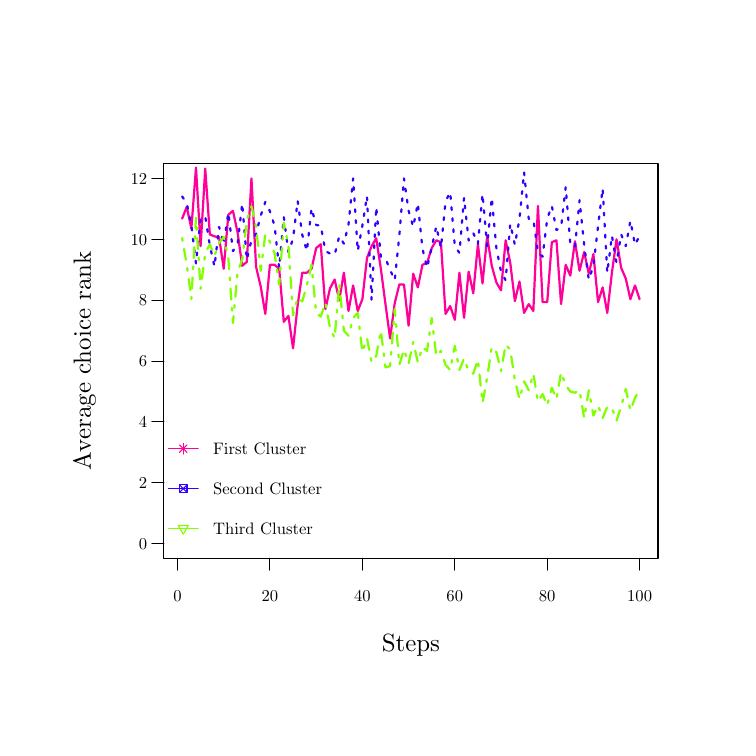
\begin{tikzpicture}[x=1pt,y=1pt]
\definecolor{fillColor}{RGB}{255,255,255}
\path[use as bounding box,fill=fillColor,fill opacity=0.00] (0,0) rectangle (252.94,252.94);
\begin{scope}
\path[clip] ( 49.20, 61.20) rectangle (227.75,203.75);
\definecolor{drawColor}{RGB}{255,0,153}

\path[draw=drawColor,line width= 0.8pt,line join=round,line cap=round] ( 55.81,183.92) --
	( 57.48,188.18) --
	( 59.15,180.37) --
	( 60.82,202.37) --
	( 62.49,173.98) --
	( 64.16,202.01) --
	( 65.83,178.24) --
	( 67.50,177.53) --
	( 69.17,177.18) --
	( 70.84,165.82) --
	( 72.51,185.34) --
	( 74.18,186.76) --
	( 75.85,178.95) --
	( 77.52,166.89) --
	( 79.19,168.31) --
	( 80.86,198.47) --
	( 82.53,166.53) --
	( 84.20,159.44) --
	( 85.87,149.50) --
	( 87.54,167.24) --
	( 89.21,167.24) --
	( 90.88,165.82) --
	( 92.55,146.66) --
	( 94.22,148.79) --
	( 95.89,137.08) --
	( 97.56,152.70) --
	( 99.23,164.40) --
	(100.90,164.40) --
	(102.57,165.82) --
	(104.24,173.27) --
	(105.91,174.69) --
	(107.58,151.28) --
	(109.25,158.73) --
	(110.92,161.92) --
	(112.59,154.47) --
	(114.26,164.40) --
	(115.93,150.57) --
	(117.60,159.79) --
	(119.27,150.57) --
	(120.94,154.82) --
	(122.61,169.73) --
	(124.28,173.98) --
	(125.95,176.82) --
	(127.62,165.82) --
	(129.29,153.05) --
	(130.96,140.63) --
	(132.63,153.41) --
	(134.30,160.15) --
	(135.97,160.15) --
	(137.64,145.25) --
	(139.31,164.05) --
	(140.98,159.08) --
	(142.65,167.24) --
	(144.32,167.95) --
	(145.99,173.27) --
	(147.66,176.11) --
	(149.33,175.40) --
	(151.00,149.50) --
	(152.67,152.34) --
	(154.34,147.37) --
	(156.01,164.40) --
	(157.68,148.08) --
	(159.35,164.76) --
	(161.02,156.95) --
	(162.69,174.69) --
	(164.36,160.50) --
	(166.03,177.53) --
	(167.70,166.89) --
	(169.37,160.86) --
	(171.04,158.02) --
	(172.71,176.11) --
	(174.38,167.95) --
	(176.05,154.12) --
	(177.71,161.21) --
	(179.38,149.86) --
	(181.05,153.05) --
	(182.72,150.57) --
	(184.39,188.53) --
	(186.06,153.76) --
	(187.73,153.76) --
	(189.40,175.40) --
	(191.07,176.11) --
	(192.74,153.05) --
	(194.41,167.24) --
	(196.08,163.34) --
	(197.75,175.76) --
	(199.42,165.11) --
	(201.09,171.86) --
	(202.76,164.05) --
	(204.43,171.15) --
	(206.10,153.76) --
	(207.77,159.08) --
	(209.44,149.86) --
	(211.11,164.40) --
	(212.78,176.47) --
	(214.45,166.18) --
	(216.12,162.28) --
	(217.79,154.82) --
	(219.46,159.79) --
	(221.13,154.82);
\end{scope}
\begin{scope}
\path[clip] (  0.00,  0.00) rectangle (252.94,252.94);
\definecolor{drawColor}{RGB}{0,0,0}

\path[draw=drawColor,line width= 0.4pt,line join=round,line cap=round] ( 54.14, 61.20) -- (221.13, 61.20);

\path[draw=drawColor,line width= 0.4pt,line join=round,line cap=round] ( 54.14, 61.20) -- ( 54.14, 56.92);

\path[draw=drawColor,line width= 0.4pt,line join=round,line cap=round] ( 87.54, 61.20) -- ( 87.54, 56.92);

\path[draw=drawColor,line width= 0.4pt,line join=round,line cap=round] (120.94, 61.20) -- (120.94, 56.92);

\path[draw=drawColor,line width= 0.4pt,line join=round,line cap=round] (154.34, 61.20) -- (154.34, 56.92);

\path[draw=drawColor,line width= 0.4pt,line join=round,line cap=round] (187.73, 61.20) -- (187.73, 56.92);

\path[draw=drawColor,line width= 0.4pt,line join=round,line cap=round] (221.13, 61.20) -- (221.13, 56.92);

\node[text=drawColor,anchor=base,inner sep=0pt, outer sep=0pt, scale=  0.60] at ( 54.14, 45.60) {0};

\node[text=drawColor,anchor=base,inner sep=0pt, outer sep=0pt, scale=  0.60] at ( 87.54, 45.60) {20};

\node[text=drawColor,anchor=base,inner sep=0pt, outer sep=0pt, scale=  0.60] at (120.94, 45.60) {40};

\node[text=drawColor,anchor=base,inner sep=0pt, outer sep=0pt, scale=  0.60] at (154.34, 45.60) {60};

\node[text=drawColor,anchor=base,inner sep=0pt, outer sep=0pt, scale=  0.60] at (187.73, 45.60) {80};

\node[text=drawColor,anchor=base,inner sep=0pt, outer sep=0pt, scale=  0.60] at (221.13, 45.60) {100};

\path[draw=drawColor,line width= 0.4pt,line join=round,line cap=round] ( 49.20, 66.48) -- ( 49.20,198.47);

\path[draw=drawColor,line width= 0.4pt,line join=round,line cap=round] ( 49.20, 66.48) -- ( 44.92, 66.48);

\path[draw=drawColor,line width= 0.4pt,line join=round,line cap=round] ( 49.20, 88.48) -- ( 44.92, 88.48);

\path[draw=drawColor,line width= 0.4pt,line join=round,line cap=round] ( 49.20,110.47) -- ( 44.92,110.47);

\path[draw=drawColor,line width= 0.4pt,line join=round,line cap=round] ( 49.20,132.47) -- ( 44.92,132.47);

\path[draw=drawColor,line width= 0.4pt,line join=round,line cap=round] ( 49.20,154.47) -- ( 44.92,154.47);

\path[draw=drawColor,line width= 0.4pt,line join=round,line cap=round] ( 49.20,176.47) -- ( 44.92,176.47);

\path[draw=drawColor,line width= 0.4pt,line join=round,line cap=round] ( 49.20,198.47) -- ( 44.92,198.47);

\node[text=drawColor,anchor=base east,inner sep=0pt, outer sep=0pt, scale=  0.60] at ( 43.20, 64.41) {0};

\node[text=drawColor,anchor=base east,inner sep=0pt, outer sep=0pt, scale=  0.60] at ( 43.20, 86.41) {2};

\node[text=drawColor,anchor=base east,inner sep=0pt, outer sep=0pt, scale=  0.60] at ( 43.20,108.41) {4};

\node[text=drawColor,anchor=base east,inner sep=0pt, outer sep=0pt, scale=  0.60] at ( 43.20,130.41) {6};

\node[text=drawColor,anchor=base east,inner sep=0pt, outer sep=0pt, scale=  0.60] at ( 43.20,152.40) {8};

\node[text=drawColor,anchor=base east,inner sep=0pt, outer sep=0pt, scale=  0.60] at ( 43.20,174.40) {10};

\node[text=drawColor,anchor=base east,inner sep=0pt, outer sep=0pt, scale=  0.60] at ( 43.20,196.40) {12};

\path[draw=drawColor,line width= 0.4pt,line join=round,line cap=round] ( 49.20, 61.20) --
	(227.75, 61.20) --
	(227.75,203.75) --
	( 49.20,203.75) --
	( 49.20, 61.20);
\end{scope}
\begin{scope}
\path[clip] (  0.00,  0.00) rectangle (252.94,252.94);
\definecolor{drawColor}{RGB}{0,0,0}

\node[text=drawColor,anchor=base,inner sep=0pt, outer sep=0pt, scale=  0.90] at (138.47, 27.60) {Steps};

\node[text=drawColor,rotate= 90.00,anchor=base,inner sep=0pt, outer sep=0pt, scale=  0.90] at ( 22.80,132.47) {Average choice rank};
\end{scope}
\begin{scope}
\path[clip] ( 49.20, 61.20) rectangle (227.75,203.75);
\definecolor{drawColor}{RGB}{51,0,255}

\path[draw=drawColor,line width= 0.8pt,dash pattern=on 1pt off 3pt ,line join=round,line cap=round] ( 55.81,191.96) --
	( 57.48,189.49) --
	( 59.15,181.41) --
	( 60.82,167.71) --
	( 62.49,184.10) --
	( 64.16,184.77) --
	( 65.83,174.22) --
	( 67.50,166.59) --
	( 69.17,180.96) --
	( 70.84,174.67) --
	( 72.51,186.12) --
	( 74.18,172.20) --
	( 75.85,174.67) --
	( 77.52,189.49) --
	( 79.19,169.06) --
	( 80.86,176.24) --
	( 82.53,178.49) --
	( 84.20,185.00) --
	( 85.87,189.94) --
	( 87.54,186.57) --
	( 89.21,181.41) --
	( 90.88,166.14) --
	( 92.55,184.55) --
	( 94.22,171.75) --
	( 95.89,176.69) --
	( 97.56,190.38) --
	( 99.23,178.04) --
	(100.90,172.20) --
	(102.57,187.69) --
	(104.24,181.63) --
	(105.91,181.41) --
	(107.58,172.20) --
	(109.25,171.31) --
	(110.92,170.86) --
	(112.59,177.59) --
	(114.26,174.90) --
	(115.93,181.86) --
	(117.60,198.47) --
	(119.27,172.20) --
	(120.94,181.41) --
	(122.61,192.18) --
	(124.28,154.47) --
	(125.95,188.14) --
	(127.62,170.18) --
	(129.29,169.51) --
	(130.96,165.47) --
	(132.63,161.65) --
	(134.30,177.81) --
	(135.97,198.47) --
	(137.64,186.79) --
	(139.31,180.96) --
	(140.98,189.49) --
	(142.65,173.10) --
	(144.32,166.14) --
	(145.99,173.55) --
	(147.66,181.18) --
	(149.33,173.33) --
	(151.00,190.16) --
	(152.67,193.53) --
	(154.34,174.00) --
	(156.01,171.53) --
	(157.68,191.51) --
	(159.35,176.02) --
	(161.02,178.71) --
	(162.69,174.90) --
	(164.36,192.85) --
	(166.03,174.00) --
	(167.70,191.51) --
	(169.37,173.33) --
	(171.04,164.80) --
	(172.71,161.65) --
	(174.38,182.08) --
	(176.05,174.45) --
	(177.71,183.88) --
	(179.38,200.71) --
	(181.05,183.88) --
	(182.72,183.65) --
	(184.39,171.98) --
	(186.06,170.18) --
	(187.73,183.88) --
	(189.40,188.59) --
	(191.07,179.83) --
	(192.74,180.73) --
	(194.41,195.32) --
	(196.08,174.90) --
	(197.75,173.55) --
	(199.42,190.61) --
	(201.09,174.45) --
	(202.76,161.88) --
	(204.43,166.82) --
	(206.10,181.18) --
	(207.77,194.87) --
	(209.44,164.35) --
	(211.11,177.81) --
	(212.78,167.94) --
	(214.45,178.26) --
	(216.12,174.00) --
	(217.79,183.20) --
	(219.46,174.45) --
	(221.13,177.81);
\definecolor{drawColor}{RGB}{128,255,0}

\path[draw=drawColor,line width= 0.8pt,dash pattern=on 1pt off 3pt on 4pt off 3pt ,line join=round,line cap=round] ( 55.81,176.93) --
	( 57.48,167.30) --
	( 59.15,154.93) --
	( 60.82,184.26) --
	( 62.49,158.59) --
	( 64.16,171.43) --
	( 65.83,174.63) --
	( 67.50,170.51) --
	( 69.17,175.09) --
	( 70.84,177.38) --
	( 72.51,169.59) --
	( 74.18,146.22) --
	( 75.85,164.55) --
	( 77.52,169.14) --
	( 79.19,183.34) --
	( 80.86,188.38) --
	( 82.53,181.05) --
	( 84.20,165.01) --
	( 85.87,178.30) --
	( 87.54,175.55) --
	( 89.21,171.43) --
	( 90.88,159.97) --
	( 92.55,182.43) --
	( 94.22,174.18) --
	( 95.89,148.97) --
	( 97.56,155.39) --
	( 99.23,154.01) --
	(100.90,159.97) --
	(102.57,167.30) --
	(104.24,149.89) --
	(105.91,148.51) --
	(107.58,153.55) --
	(109.25,144.39) --
	(110.92,140.72) --
	(112.59,160.43) --
	(114.26,143.47) --
	(115.93,141.64) --
	(117.60,148.05) --
	(119.27,149.89) --
	(120.94,135.68) --
	(122.61,140.72) --
	(124.28,132.01) --
	(125.95,134.31) --
	(127.62,143.47) --
	(129.29,130.18) --
	(130.96,130.64) --
	(132.63,151.26) --
	(134.30,131.10) --
	(135.97,136.60) --
	(137.64,131.56) --
	(139.31,139.35) --
	(140.98,132.01) --
	(142.65,137.51) --
	(144.32,136.14) --
	(145.99,148.05) --
	(147.66,134.31) --
	(149.33,136.14) --
	(151.00,131.10) --
	(152.67,129.26) --
	(154.34,137.97) --
	(156.01,129.26) --
	(157.68,133.39) --
	(159.35,128.81) --
	(161.02,127.89) --
	(162.69,132.93) --
	(164.36,117.35) --
	(166.03,126.51) --
	(167.70,137.51) --
	(169.37,135.68) --
	(171.04,128.81) --
	(172.71,138.43) --
	(174.38,136.60) --
	(176.05,125.60) --
	(177.71,118.72) --
	(179.38,125.14) --
	(181.05,121.93) --
	(182.72,127.89) --
	(184.39,117.81) --
	(186.06,120.56) --
	(187.73,116.43) --
	(189.40,122.85) --
	(191.07,118.72) --
	(192.74,128.35) --
	(194.41,123.77) --
	(196.08,121.47) --
	(197.75,121.02) --
	(199.42,121.93) --
	(201.09,111.85) --
	(202.76,121.93) --
	(204.43,112.77) --
	(206.10,116.43) --
	(207.77,111.85) --
	(209.44,115.97) --
	(211.11,115.52) --
	(212.78,110.93) --
	(214.45,115.97) --
	(216.12,122.39) --
	(217.79,114.60) --
	(219.46,119.18) --
	(221.13,121.93);
\definecolor{drawColor}{RGB}{255,0,153}

\path[draw=drawColor,line width= 0.4pt,line join=round,line cap=round] ( 50.82,100.80) -- ( 61.62,100.80);
\definecolor{drawColor}{RGB}{51,0,255}

\path[draw=drawColor,line width= 0.4pt,line join=round,line cap=round] ( 50.82, 86.40) -- ( 61.62, 86.40);
\definecolor{drawColor}{RGB}{128,255,0}

\path[draw=drawColor,line width= 0.4pt,line join=round,line cap=round] ( 50.82, 72.00) -- ( 61.62, 72.00);
\definecolor{drawColor}{RGB}{255,0,153}

\path[draw=drawColor,line width= 0.4pt,line join=round,line cap=round] ( 54.87, 99.45) -- ( 57.57,102.15);

\path[draw=drawColor,line width= 0.4pt,line join=round,line cap=round] ( 54.87,102.15) -- ( 57.57, 99.45);

\path[draw=drawColor,line width= 0.4pt,line join=round,line cap=round] ( 54.31,100.80) -- ( 58.13,100.80);

\path[draw=drawColor,line width= 0.4pt,line join=round,line cap=round] ( 56.22, 98.89) -- ( 56.22,102.71);
\definecolor{drawColor}{RGB}{51,0,255}

\path[draw=drawColor,line width= 0.4pt,line join=round,line cap=round] ( 54.87, 85.05) rectangle ( 57.57, 87.75);

\path[draw=drawColor,line width= 0.4pt,line join=round,line cap=round] ( 54.87, 85.05) -- ( 57.57, 87.75);

\path[draw=drawColor,line width= 0.4pt,line join=round,line cap=round] ( 54.87, 87.75) -- ( 57.57, 85.05);
\definecolor{drawColor}{RGB}{128,255,0}

\path[draw=drawColor,line width= 0.4pt,line join=round,line cap=round] ( 56.22, 69.90) --
	( 58.04, 73.05) --
	( 54.40, 73.05) --
	( 56.22, 69.90);
\definecolor{drawColor}{RGB}{0,0,0}

\node[text=drawColor,anchor=base west,inner sep=0pt, outer sep=0pt, scale=  0.60] at ( 67.02, 98.73) {First Cluster};

\node[text=drawColor,anchor=base west,inner sep=0pt, outer sep=0pt, scale=  0.60] at ( 67.02, 84.33) {Second Cluster};

\node[text=drawColor,anchor=base west,inner sep=0pt, outer sep=0pt, scale=  0.60] at ( 67.02, 69.93) {Third Cluster};
\end{scope}
\end{tikzpicture}

\end{frame}


\begin{frame}{Experiment Results}
	\framesubtitle{IGT data for conviceted criminals}
	\setbeamertemplate{itemize items}[circle]
	Authors results:
	\begin{itemize}
		\item Specialized version IGT test
		\item No control group
		\item EVM analysis shows clustering for convicted robbery and assault/murders; Other criminal groups have overlapping parameters
	\end{itemize}
		Our findings:
		\begin{itemize}
			\item Convicted assault/murders separate the strongest (highest clustering against forgery)
			\item Robbery only cluster moderately in our settings
		\end{itemize}
\end{frame}

\begin{frame}{Experiment Results}
	\framesubtitle{IGT data for drug abusers}
	\setbeamertemplate{itemize items}[circle]
	Author's findings
	\begin{itemize}
		\item Cocaine abusers persistently do disadvantageous choices
		\item Effect still present after controlling for IQ (in general lower than within control group)
	\end{itemize}
	Our findings
	\begin{itemize}
		\item Only moderate clustering between control group and cocaine abusers
		\item Best separation criteria turned out disadvantageous behaviour
	\end{itemize}
\end{frame}


\begin{frame}{Conclusion}
	\setbeamertemplate{itemize items}[circle]
	Key - Finings
	\begin{itemize}
		\item Clustering peoples choices in general difficult
		\item Algorithms can recover clustering if individuals show sufficient difference in their strategic behaviour
	\end{itemize}
	
\end{frame}

\end{document}